\documentclass[a4paper,10pt]{article}
\usepackage[utf8]{inputenc}
\usepackage{amsmath}
\usepackage{graphicx}
\usepackage{geometry}
\usepackage{setspace}
\geometry{top=0.5in, bottom=0.5in, left=0.5in, right=0.5in}
\setstretch{1} 
\title{\textbf{Analysis of Key West Annual Mean Temperature}}
\author{Yaxin Liu}
\date{04/12/2024}
\begin{document}

\maketitle
\section*{Introduction}
This report analyzes the annual mean temperature data for Key West to investigate the relationship between year and temperature. A statistical test is performed to determine whether the observed correlation coefficient between year and temperature is statistically significant. A permutation test is employed to assess the significance.
\section*{Results}
The analysis yielded the following results:
\begin{itemize}
    \item \textbf{Observed Correlation:} The correlation coefficient between year and temperature was:
    \[
    r = 0.53
    \]
    \item \textbf{Permutation Test:} Based on 5000 randomizations, the p-value was:
    \[
    p = 0
    \]
\end{itemize}
\begin{figure}[h!]
    \centering
    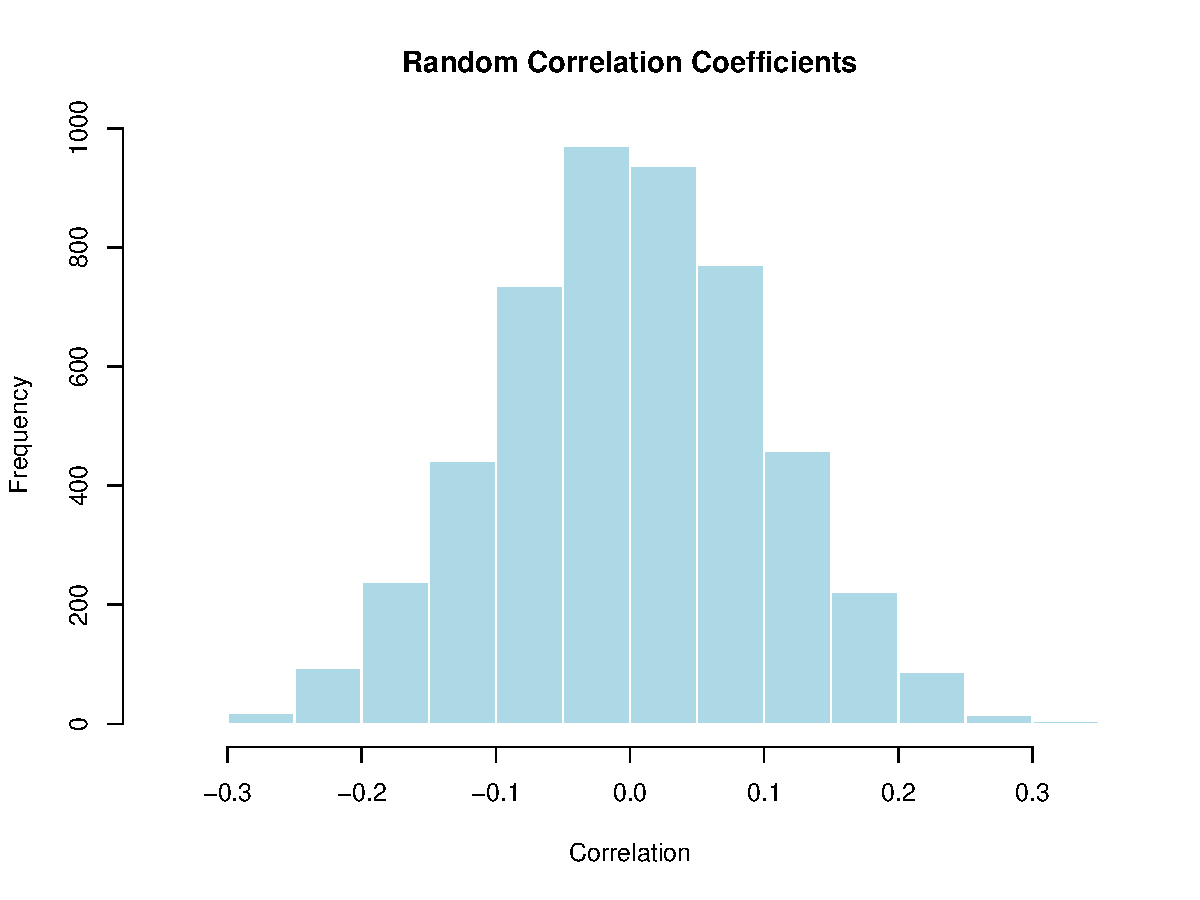
\includegraphics[width=0.5\textwidth, height=0.3\textheight]{../results/Florida.pdf}
    \caption{Histogram of correlation coefficients from 5000 permutations. The red dashed line represents the observed correlation.}
    \label{fig:histogram}
\end{figure}
\section*{Conclusion}
The results indicate that the observed correlation between year and temperature is statistically significant (\(p = 0\)), suggesting that the increasing trend in temperatures over the years is unlikely to be due to random variation. The histogram highlights the rarity of random correlations exceeding the observed correlation coefficient.
\immediate\write18{mv FloridaLatexCode.pdf ../results/}
\end{document}
